\documentclass{article}
\usepackage{nips07submit_e,times}
%\documentstyle[nips07submit_09,times]{article}

\usepackage{amsmath,amsthm,amssymb}
\usepackage{graphicx}


\newtheorem{theorem}{Theorem}
\newtheorem{lemma}{Lemma}
\newtheorem{corollary} {Corollary}
\newtheorem{definition} {Definition}
\newtheorem{example} {Example}
\newtheorem{examplelemma} {Example Lemma}
\newtheorem{exampletheorem} {Example Theorem}

\newcommand{\maybekillspace}{\vspace{-0.08in}}
\newcommand{\killspace}{\vspace{-0.08in}}
\newcommand{\killproofspace}{\vspace{-0.08in}}
\newcommand{\mysection}[1]{\vspace{-0.04in}\section{#1}\killspace}

\newcommand{\GNP}[1][\psi]{{#1}_{\Theta}}
\newcommand{\GNPvec}[1][\psi]{{#1}_{\overrightarrow{\Theta}}}

\newcommand{\otimesvec}{\mathbin{\overrightarrow{\otimes}}}
\newcommand{\odotvec}{\mathbin{\overrightarrow{\odot}}}
\newcommand{\bigotimesvec}{\mathop{\overrightarrow{\bigotimes}}}
\newcommand{\bigodotvec}{\mathop{\overrightarrow{\bigodot}}}

\newcommand{\sigmahat}{\mathbin{\widehat{\sigma}}}
\newcommand{\otimeshat}{\mathbin{\widehat{\otimes}}}
\newcommand{\odothat}{\mathbin{\widehat{\odot}}}
\newcommand{\bigotimeshat}{\mathop{\widehat{\bigotimes}}}
\newcommand{\bigodothat}{\mathop{\widehat{\bigodot}}}

\newcommand{\otimestilde}{\mathbin{\widetilde{\otimes}}}
\newcommand{\odottilde}{\mathbin{\widetilde{\odot}}}
\newcommand{\bigotimestilde}{\mathop{\widetilde{\bigotimes}}}
\newcommand{\bigodottilde}{\mathop{\widetilde{\bigodot}}}

\DeclareMathOperator*{\argmin}{argmin}
\DeclareMathOperator*{\argmax}{argmax}
\DeclareMathOperator*{\map}{map}
\DeclareMathOperator*{\minmax}{minmax}
\DeclareMathOperator{\sign}{sign}
\DeclareMathOperator{\prunes}{prunes}

\DeclareMathOperator{\leftchild}{left}
\DeclareMathOperator{\rightchild}{right}
\DeclareMathOperator{\parent}{parent}
\DeclareMathOperator{\sibling}{sibling}
\DeclareMathOperator{\op}{op}

\newcommand{\comp}{\mathbin{\circ}}
\newcommand{\st}{{\rm~s.t.~}}

% Useful commands
\newcommand{\fig}[1]{Figure~\ref{fig:#1}}

% Standardized pseudocode functions
%\newcommand{\dist}[2]{||#1-#2||}
\newcommand{\spos}{^{{\scriptscriptstyle +\!}}}
\newcommand{\sneg}{^{{\scriptscriptstyle -\!}}}

\newcommand{\disthrectmin}{d^{l}}
\newcommand{\disthrectmax}{d^{u}}
\newcommand{\dist}[2]{d(#1,#2)}
\newcommand{\kdroot}[1]{#1^{\text{\rm root}}}
\newcommand{\kdleft}[1]{#1^{\!L}}
\newcommand{\kdright}[1]{#1^{\!R}}

\newcommand{\simhrectmin}{S^{l}}
\newcommand{\simhrectmax}{S^{u}}

\newcommand{\al}{a^l}
\newcommand{\au}{a^u}
\newcommand{\dl}{d^l}
\newcommand{\du}{d^u}

% Spacing for standardized pseudocode
\newcommand{\X}{\\ \scriptstyle}
\newcommand{\x}{\\ \hspace{0.13in} \scriptstyle}
\newcommand{\xx}{\\ \hspace{0.26in} \scriptstyle}
\newcommand{\xxx}{\\ \hspace{0.39in} \scriptstyle}
\newcommand{\xxxx}{\\ \hspace{0.52in} \scriptstyle}

% Variables for affinity propagation
\newcommand{\eqspace}{\!\!\!\!}
\newcommand{\true}{\text{true}}
\newcommand{\ocpos}[1]{c^{+}_{#1}}
\newcommand{\ocneg}[1]{c^{-}_{#1}}
\newcommand{\cpos}[2]{\ocpos{#1 \neq #2}}
\newcommand{\cneg}[2]{\ocneg{#1 \neq #2}}

\newcommand{\intersect}{\cap}

\newcommand{\respo}[2]{R_{#1#2}}
\newcommand{\avail}[2]{A_{#1#2}}
\newcommand{\simil}[2]{S_{#1#2}}

\newcommand{\vecrho}{\vec{\rho}}
\newcommand{\vecalpha}{\vec{\alpha}}
\newcommand{\frho}[1]{\rho_{#1}}
\newcommand{\falpha}[1]{\alpha_{#1}}
\newcommand{\falphaj}[2]{\alpha_{#1[#2]}}

\newcommand{\falphamax}{\alpha^{u}}
\newcommand{\falphamin}{\alpha^{l}}
\newcommand{\frhomax}{\rho^{u}}
\newcommand{\frhomin}{\rho^{l}}

\newcommand{\alphacand}{v}

\newcommand{\ignoreall}[1]{}

\title{A Mathematical Theory for Scalable Learning}

\author{
Ryan N.~Riegel \\
College of Computiong \\
Georgia Institute of Technology \\
Atlanta, GA 30332 \\
\texttt{rriegel@cc.gatech.edu} \\
\And
Garrett F.~Boyer \\
College of Computiong \\
Georgia Institute of Technology \\
Atlanta, GA 30332 \\
\texttt{garryb@cc.gatech.edu} \\
\And
Alexander G.~Gray \\
College of Computiong \\
Georgia Institute of Technology \\
Atlanta, GA 30332 \\
\texttt{agray@cc.gatech.edu} \\
}

% The \author macro works with any number of authors. There are two commands
% used to separate the names and addresses of multiple authors: \And and \AND.
%
% Using \And between authors leaves it to \LaTeX{} to determine where to break
% the lines. Using \AND forces a linebreak at that point. So, if \LaTeX{}
% puts 3 of 4 authors names on the first line, and the last on the second
% line, try using \AND instead of \And before the third author name.

\begin{document}

\makeanontitle

\begin{abstract}
We present mathematical foundations for a highly successful
algorithmic strategy that has resulted in the fastest algorithms for
many machine learning methods and is broadly applicable to scaling
many future methods up to large datasets.  We formalize for the first
time a class of computational problems which are common in machine
learning, called {\em generalized $N$-body problems} (GNP's), and
provide a calculus for simplification of GNP's in various ways.  We
then present a template {\em generalized $N$-body algorithm} applying
to any GNP, which can be specialized to mathematically derive
efficient problem-dependent algorithms using the calculus.  We
demonstrate the use of this mathematical framework for deriving a fast
algorithm for the recent affinity propagation method.
\end{abstract}

\mysection{Introduction}

The ability to apply machine learning methods to large datasets is
increasingly important for many applications.  Unfortunately,
powerful nonparametric methods are commonly $O(N^2)$ or
$O(N^3)$, where there are $O(N)$ test (or query) points and training
(or reference) points.
The authors of \cite{nips2000paper} presented a new algorithmic strategy
based on the simultaneous traversal of multiple space-partitioning
trees, which applies to a number of machine learning methods.  The set
of problems to which this strategy is applicable was informally named
{\em generalized $N$-body problems}, in reference to breakthrough
methods for computational physics problems \cite{appel2,barnes_hut,grngard}
which can be seen as special cases.
%all of which have the same
%characteristic form.  This algorithmic strategy generalizes other
%successful algorithms for specific problems in addition to these
%physics problems, such as computing the well-separated pair
%decomposition in theoretical computer science [[wspd]], computing the
%spatial join in databases [[spatial join]], and computing set
%intersections [[baeza-yates]].  In each of these problems no superior
%algorithmic strategy is known.
% also a kind of dual-tree method in graphics for object collision
% detection, but we need the reference
This multi-tree algorithmic strategy has been applied to a succession
of well-known statistical learning methods, each representing certain
unique challenges for the strategy, including
all-$k$-nearest-neighbors (a generalization of $k$-nearest-neighbors)
\cite{nips2000paper}, kernel density estimation \cite{nips2000paper,
kde-siamdm, kde-aistats, kde-nips-dong, kde-uai-dong},
$k$-nearest-neighbor classification \cite{ting-liu}, kernel discriminant
analysis (or nonparametric Bayes classification) [[nbc-phystat,
\cite{nbc-compstat}]], and $n$-point correlation functions [[\cite{nips2000paper,
moore-npt}, npt-2004]].  These algorithms have been demonstrated on
large scientific datasets, producing first-of-a-kind high-profile
results, e.g.~\cite{science03, nature05}.  For each of these
problems, no overall faster algorithms are known.  Other machine
learning problems which have been treated using this strategy include
dimensionality reduction methods \cite{hochreiter00beyond}, nonparametric
belief propagation \cite{alex-ihler}, multiple tracking \cite{kbc:stch}, linear algebraic machine learning methods \cite{freitas_fast},
and particle filters \cite{klaas_fast, klaas-toward, klaas-fast}.
Many other current and future machine learning methods remain to be
treated in depth with this strategy, not to mention a large array of
related fundamental problems in computational geometry, physics, and
applied mathematics.  

This paper treats two basic questions: 1) What
is the scope of the problems to which this methodology can be applied? 2)
How can the successful ideas which have been developed over many problem 
examples be expertly applied by new researchers wishing to
design fast algorithms for future machine learning methods?
To make the ideas concrete, we begin with examples of some problems
and corresponding algorithms resulting from our approach.  We then
mathematically formalize the class of {\em generalized $N$-body
problems} (GNP's) for the first time.  We also formalize the
algorithmic approach as a single generic algorithm, {\em the
generalized $N$-body algorithm}, which can be specialized to any problem in the
class, possibly automatically \cite{autobayes}.
We elucidate some of
the abstract mathematical properties of such problems that can be
exploited to achieve computational efficiency, through a number of
lemmas forming a calculus of transformations of GNP's.  We then return
to our examples and demonstrate the derivation of each algorithm using
our calculus.  As a more sophisticated final example, we apply the
theory to derive a fast algorithm for as recent a method as we could
find, the affinity propagation method of clustering \cite{affinity}, and
demonstrate its efficiency.

%\footnote{Beyond facilitating application by
%humans to new problems, we strive for a level of precise specification
%which goes even farther, opening up the possibility of automatic
%derivation of algorithms for new problems [[autobayes]], as did the
%specification of the generic EM algorithm by [[dempster et al.]].}

%Aside from speed,
%a unique advantage of this algorithmic approach is the ability to
%specify and achieve rigorous relative error tolerances when
%approximation is necessary, contrary to virtually all other
%approximate speedup approaches.  

%Nando de Freitas, Yang Wang, Maryam Mahdaviani and Dustin Lang. Fast
%Krylov Methods for N-Body Learning . NIPS 2005.
%
%Mike Klaas, Dustin Lang and Nando de Freitas. Fast Maximum a
%Posteriori Inference in Monte Carlo State Spaces . AISTATS 2005.
%
%Mike Klaas, Nando de Freitas and Arnaud Doucet. Toward Practical N^2
%Monte Carlo: The Marginal Particle Filter . UAI 2005
%
%Mike Klaas, Mark Briers, Nando de Freitas, Arnaud Doucet, Simon
%Maskell and Dustin Lang. Fast Particle Smoothing: If I Had a Million
%Particles. ICML 2006. 
%
%inproceedings{ hochreiter00beyond,
%    author = "Sepp Hochreiter and Michael Mozer",
%    title = "Beyond Maximum Likelihood and Density Estimation: A Sample-Based Criterion for Unsupervised Learning of Complex Models",
%    booktitle = "{NIPS}",
%    pages = "535-541",
%    year = "2000",
%    url = "citeseer.ist.psu.edu/541475.html" }

%Some fundamental problems to which the multi-tree strategy is
%applicable are shown in Figure~\ref{tab:probs}, including some canonical
%problems in theoretical computer science [[preparata-shamos]].  These
%problems commonly occur in many guises in many fields, including many
%machine learning methods, both classical and modern, such as recent
%manifold learning [[lle, isomap]] methods.

%In the next section, to make the ideas concrete, we present one of the
%more easily understood problems in our class and an efficient
%multi-tree method for it.  We then define generalized $N$-body
%problems, and show that they have a decomposability property which
%ultimately admits a general recursive formulation, the generalized
%$N$-body algorithm.  Making the generalized $N$-body algorithm
%efficient requires a problem-dependent pruning step.  The following
%two sections discuss problem-dependent properties which admit
%efficient pruning steps in the cases of exact and approximate
%computation, respectively.  We conclude with examples of designing
%fast algorithms for machine learning problems, starting with the
%problem of nonparametric density thresholding, a common folk method
%for anomaly detection.  Finally, as a demonstration of the practical
%relevance of this methodology to state-of-the-art machine learning
%methods, we considered the most recent method we could find, affinity
%propagation [[affinity]], and designed and implemented in one day a
%fast algorithm for it allowing it to scale to large datasets despite
%its straightforward $O(N^2)$ runtime.

\mysection{Examples}

% Begin figure

\begin{figure}
  \begin{minipage}{1.8in}
    \begin{minipage}{0.8in}
      \includegraphics[width=0.75in,height=1.0in]{kdtree-level2.ps}
    \end{minipage}
    \begin{minipage}{0.8in}
      \includegraphics[width=0.75in,height=1.0in]{kdtree-level4.ps}
    \end{minipage}
    \\
    \begin{minipage}{1.6in}
      \footnotesize{\caption{A two-dimensional $kd$-tree at (left) level 2 and (right) level 4.}}
    \end{minipage}
  \end{minipage}
  \label{fig:kdtree}
\end{figure}
\begin{figure}
  \vspace{-1.89in}
  \hspace{1.8in}
  %\begin{minipage}{2.8in}
  %\end{minipage}
  \begin{minipage}{3.88in}
    \begin{minipage}{1.8in}
      \begin{displaymath}
      %\hspace{-0.17in}
      %\begin{array}{l}
        \begin{array}{l}
          \text{{\bf tpc} - Two-point correlation.}
          \X \text{function tpc}(Q, R)
          \x \text{if }\disthrectmax(Y, X) < r\text{: return }0
          \x \text{if }\disthrectmin(Y, Y) > r\text{: return } |Y| \cdot |X|
          \x \text{elif }|Y| \geq |X|\text{:}
          \xx \text{return tpc}(\kdleft{Y}, X, r) + \text{tpc}(\kdright{Y}, X, r)
          \x \text{else:}
          \xx \text{return tpc}(Y, \kdleft{X}, r) + \text{tpc}(Y, \kdright{X}, r)
        \end{array}
       \end{displaymath}
       \vspace{-.11in}
       \caption{\label{fig:allnntpc}\footnotesize Pseudocode for two simple dual-tree algorithms.}
      \end{minipage}
      \begin{minipage}{2.0in}
       \begin{displaymath}
        \begin{array}{l}
          \text{{\bf allnn} - All-nearest-neighbors.}
          \X \text{init all nodes }Q \subseteq \kdroot{Q}\text{: }a(Q) \gets \infty
          \X \text{procedure allnn}(Q,R)\text{:}
          \x \text{if }a(Q) < \disthrectmin(Q, R)\text{: return}
          \x \text{elif }Q = \{q\} \text{ and } R = \{r\}
          \xx a(\{q\}) \gets \min(a(\{q\}), \dist{Q}{R})
          \x \text{elif }|Q| \geq |R|\text{:}
          \xx \text{allnn}(\kdleft{Q}, R); \text{ allnn}(\kdright{Q}, R)
          \xx a(Q) \gets \max(a(\kdleft{Q}), a(\kdright{Q}))
          \x \text{else prioritize by min distance:}
          \xx \text{allnn}(Q, \kdleft{R}); \text{ allnn}(Q, \kdright{R})
          \\
        \end{array}
       \end{displaymath}
      \end{minipage}
      %\end{array}
%       &
%       \hspace{-0.2in}
%       \begin{array}{l}
%         \text{{\bf nbc} - Nonparametric Bayes classification}
%         \\ \text{init all nodes }Q \subseteq \kdroot{Q}\text{: }a(Q) \gets (0, 0)
%         \\ P \gets \text{new priority queue};~\text{postpone}(\kdroot{Q}, \kdroot{R})
%         \\ \text{while } P \text{ not empty}
%         \x (Q, R, \dl, \du) \gets \text{pop maximum from }P
%         \x \forall Q' \subseteq Q,~ \au(Q') \gets \max(\au(\kdleft{Q}), \au(\kdright{Q}))
%         \x \forall Q' \subseteq Q,~ \al(Q') \gets \min(\al(\kdleft{Q}), \al(\kdright{Q}))
%         \x \text{if }\al(Q) > 0\text{: label all points in }Q\text{ positive}
%         \x \text{elif }\au(Q) < 0\text{: label all points in }Q\text{ negative}
%         \x \text{else:}
%         \xx \text{recursively, }a(Q') \gets a(Q') - (\dl, \du)
%         \xx \text{postpone}(\kdleft{Q}, \kdleft{R}); \text{ postpone}(\kdleft{Q}, \kdright{R})
%         \xx \text{postpone}(\kdright{Q}, \kdleft{R}); \text{ postpone}(\kdright{Q}, \kdright{R})
%         \\
%         \\ \text{procedure postpone}(Q, R)\text{:}
%         \x \dl \gets \pi\spos|R\spos|K^{u}(Q, R\spos) + \pi\sneg|R\sneg|K^{l}(Q, R\sneg)
%         \x \du \gets \pi\spos|R\spos|K^{l}(Q, R\spos) + \pi\sneg|R\sneg|K^{u}(Q, R\sneg)
%         \x \forall Q' \subset Q,~ a(Q') \gets a(Q') + (\dl, \du)
%         \x \text{place }(Q, R, \dl, \du)\text{ in }P\text{ at priority }(\du-\dl)
%         \\
%         \\
%       \end{array}
  \end{minipage}
  \vspace{-.2in}
\end{figure}
Here, we present two simple dual-tree algorithms, two-point correlation and all-nearest-neighbors.
%, and nonparametric Bayes classification.
We use spatial trees, where every node $X$ in tree $\kdroot{X}$ is a set of points; every internal node is partitioned $\kdleft{X} \cup \kdright{X} = X$, with each leaf a single point $\{x\}$.
For example, a $kd$-tree, as in Figure~\ref{fig:kdtree}, recursively partitions the data along coordinate dimensions.
We also denote $d$ to be a distance metric, and superscripts $l$ and $u$ to refer respectively to lower and upper bounds.

{\bf The Two-point Correlation.} As a member of the family of $n$-point correlation functions, collectively the foundation for all spatial statistics, the two-point correlation\footnote{The number of non-redundant pairs may be computed as an algebraic post-processing step.} of data set $X$ for radius $r$ is
$\sum_{y \in X} \sum_{x \in X} I(d(y, x) \leq r)$ for the indicator function $I$.
\fig{allnntpc} shows a formulation that recursively considers a subset pair $Y$ and $X$, returning immediately if all points in $Y$ and $X$ are completely inside or outside the radius.

{\bf All-nearest-neighbors.} In applications from manifold learning to computational physics, it is often desirable to find for a batch of queries $Q$ the nearest neighbors from reference set $R$, as $\map_{q \in Q} \argmin_{r \in R} d(q,r)$, with the exception $d(q,q) = \infty$.
To achieve speedup, one maintains for each recursive subset of queries the furthest candidate neighbor distance found.
If a considered set of references is farther away than this distance, no further exploration is required.

% {\bf Nonparametric Bayes Classification.}
% A simple kernel-based classifier labels each point in $Q$ positive or negative by weighing the density generated by a kernel at each training example in $R\spos$ and $R\sneg$, weighed respectively by priors $\pi\spos$ and $\pi\sneg$:
% \begin{equation*}
% \map_{q \in Q} I\Big(\sum_{r \in R\spos} \pi\spos K(q,r) - \sum_{r \in R\sneg} \pi\sneg K(q,r) \geq 0 \Big)
% \end{equation*}
% \noindent for distance-based kernel $K$.
% Each subset of queries maintains an upper and lower bound on the difference of the sums, and is labelled when this range no longer contains zero.
% A simple non-recursive algorithm uses a priority queue, relying on the fact that iterating over all children is quite inexpensive compared to the recursion\footnote{In practice, some of these updates may be performed lazily.}.

%  The all-nearest-neighbors problem (All-NN) aims to find for each
%  point in some set $Q$ of queries the nearest point from a set $R$ of
%  references, possibly identical to $Q$.  The problem is represented
%  mathematically as
%  \[
%  \map_{1 \leq i \leq |Q|}\argmin_{1 \leq j \leq |R|} d(q_i,r_j),
%  \]
%  where metric $d(q_i,r_i) \equiv \infty$ if $Q = R$.
%  
%  [[Examples of uses.]]
%  
%  All-NN is solved efficiently by Algorithm~\ref{alg:all-nn}, which
%  works on trees formed for both queries and references.  It maintains
%  for each query node an upper bound on the distance to any of its
%  points' nearest neighbors; in short, the maximum distance to any
%  candidate nearest neighbor seen so far.  When a pair of query and
%  reference nodes have a lower-bound distance greater than the query
%  node's stored upper bound, it is impossible for the reference node to
%  contribute any of the contained queries' nearest neighbors and all
%  work between the nodes may be pruned.
%  
%  \subsection{Kernel Density Estimation}
%  
%  Kernel Density Estimation (KDE) wraps a small probability density
%  function around each point in some data set in order to estimate that
%  set's distribution.  It is then of interest to determine each point's
%  density in order to detect outliers.  Alternately, we may find
%  densities for a set of queries not from the original data set.
%  \[
%  \map_{q \in Q} \sum_{r \in R} K_h(q,r).
%  \]
%  [[Perhaps mention fitting bandwidth with LOO and L2E, etc.]]
%  
%  \subsection{Nonparametric Bayes Classification}
%  
%  Nonparametric Bayes classification (NBC) applies Bayes' Rule to the
%  results of kernel density estimation in order to predict the class of
%  each of some set of queries $Q$ given sets of references $R_k$ for
%  classes $C_k$, $1 \leq k \leq M$.  The problem is given by
%  \[
%  \map_{1 \leq i \leq |Q|} \argmax_{1 \leq k \leq M} \sum_{1 \leq j \leq |R_k|} K_{h_k}(q_i,r_j),
%  \]
%  where $K(q_i,r_i) \equiv 0$ if $Q = R$, permitting computation for
%  leave-one-out cross-validation.
%  
%  [[Examples of uses.]]
%  
%  Algorithm~\ref{alg:nbc} demonstrate an efficient means of computing
%  NBC in the two-class case.  It forms trees for all involved sets and
%  maintains at query nodes both upper and lower bounds on density
%  contributions from the various classes.  When one class's lower-bound
%  joint probability (found by multiplying the class's lower-bound
%  density and prior) is greater than all other's upper-bounds, then we
%  may safely conclude that all queries within the node should be
%  attributed to that class.
%  
%  \subsection{Multi-radius $n$-point Correlation}
%  
%  The $n$-point correlation is found by counting all unique $n$-tuples
%  of points within some radius $r$ of one another.  It is found with
%  \[
%  \sum_{x_{i_1} \in X} \cdots \sum_{x_{i_n} \in X} I(d(x_{i_j},x_{i_k}) < r \forall j,k),
%  \]
%  where $I(d(x_{i_j},x_{i_k}) < r \forall j,k) \equiv 0$ unless $i_1 <
%  \cdots < i_n$.
%  
%  [[Examples of uses.]]
%  
%  [[Description of algorithm.]]

%%%%%%%%%%%%%%%%%%%%%%%%%%%%%%%%%%%%%%%%%%%%%%%%%%%%%%%%%%%%%%%%%%%%%%%%%%%%%%%
\mysection{Generalized $N$-body Problems}

The class of Generalized $N$-body Problems (GNPs), exemplified above,
%or problems solvable by means similar to those shown above,
is a subset of the problems representable as nested applications of high-order function
reduce.  Reduce is a long-standing and highly versatile feature of
functional programming languages, traditionally operating over a list
from beginning to end or vice versa.  We pose reduce as a function on
unordered input multisets\footnote{Unless otherwise noted, data sets
are understood to be finite multisets, thereby permitting entries with
identical values; alternately, data sets may store a distinct index
for each entry, rendering all entries unique.} rather than lists, and
allow for pre- and postprocessing functions.
\begin{definition}
  A {\bf first-order reduce problem} $\theta$ is a tuple
  $(\mathcal{X},\otimes,f,g)$ of set of possible inputs $\mathcal{X}$,
  commmutative, associative operator $\otimes \colon \mathcal{A}
  \times \mathcal{A} \to \mathcal{A}$, and functions $f \colon
  \mathcal{X} \to \mathcal{A}$ and $g \colon \mathcal{A} \to
  \mathcal{B}$.  Its components form $\Psi_{\theta} = g \comp
  \psi_{\theta}$, where $\psi_{\theta}(X) = \bigotimes_{x \in X} f(x)$
  for nonempty $X \subset \mathcal{X}$.
\end{definition}
\killspace
\noindent The operators involved in reduce problems form abelian
semigroups; frequently, they also have identities and inverses in
$\mathcal{A}$, thereby forming abelian groups.

\begin{example}
  The expected value of a function under a sampled distribution,
  $\frac{1}{N} \sum_{x \in X} f(x)$, is a first-order reduce problem.
\end{example}
\killspace
The inner functions of reduce problems may themselves be reduce
problems, for example with $f_1(x) = \Psi_{\theta_2}(X_2)$.  While the
methods presented below can potentially extend to arbitrary nesting
depth, this paper focuses on second-order problems, or problems of two
operators.
\begin{definition}
  A {\bf second-order reduce problem} $\Theta$ is a tuple
  $(\mathcal{X},\mathcal{Y},\otimes,\odot,f,g,h)$ of sets of possible
  inputs $\mathcal{X}$ and $\mathcal{Y}$, commutative, associative
  operators $\otimes \colon \mathcal{A} \times \mathcal{A} \to
  \mathcal{A}$ and $\odot \colon \mathcal{B} \times \mathcal{B} \to
  \mathcal{B}$, and functions $f \colon \mathcal{X} \times \mathcal{Y}
  \to \mathcal{A}$, $g \colon \mathcal{Y} \times \mathcal{A} \to
  \mathcal{B}$, and $h \colon \mathcal{B} \to \mathcal{C}$.  Its
  components form $\Psi_{\Theta} = h \comp \psi_{\Theta}$, where
  $\psi_{\Theta}(Y,X) = \bigodot_{y \in Y} g \left( y,\bigotimes_{x
  \in X} f(x,y) \right)$ for nonempty $X \subset \mathcal{X}$ and $Y
  \subset \mathcal{Y}$.
\end{definition}
\killspace
\noindent The results of second-order reduce problems may be found
na\"{\i}vely through nested iteration.  If involved functions are
constant time and $X$ and $Y$ are $O(N)$, this method of computation
is $O(N^2)$.
% which is infeasible for large $N$.
\begin{example}
  The log-likelihood of a mixture of Gaussians, $\sum_{x \in X} \log
  \sum_{k \in C} \omega_k \phi(x | \mu_k, \Sigma_k)$ is a second-order
  reduce problem.
\end{example}
\killspace
Certain constraints are required by the algorithmic technique
presented in the next section, though we will later introduce a
transform to help work around them.
\begin{definition}
  Second-order reduce problem $\Theta$ is {\bf regular} if $g(y,a) =
  a$ for all $y \in \mathcal{Y}$ and $a \in \mathcal{A}$, and is thus
  given by $\Psi_{\Theta} = h \comp \psi_{\Theta}$, where
  $\psi_{\Theta}(Y,X) = \bigodot_{y \in Y} \bigotimes_{x \in X}
  f(x,y)$.  Note that $\mathcal{B} = \mathcal{A}$.
\end{definition}
\begin{definition}
  Regular second-order reduce problem $\Theta$ is {\bf block
  decomposable} if, for all nonempty partitions $\kdleft{X} \cup \kdright{X}
  = X \subset \mathcal{X}$ and nonempty $Y \in \mathcal{Y}$,
  $\GNP(Y,X) = \GNP(Y,\kdleft{X}) \otimes \GNP(Y,\kdright{X})$.  Such a
  problem\footnote{Observe that commutativity and associativity ensure
  that $\GNP(Y,X) = \GNP(\kdleft{Y},X) \odot \GNP(\kdright{Y},X)$.} is known
  as a {\bf second-order generalized $N$-body problem}.
\end{definition}

% \subsection{The Map Operator}
\maybekillspace
{\bf The Map Operator.}  High-order function map is suitable for all
problems that compute separate results for some set of queries and may
help with some problems that do not.  Reduce problems subsume the
functionality of map with $\map_{x \in X} f(x) \equiv \bigcup_{x \in
X} \{(x,f(x))\} = \{(x,f(x)) | x \in X\}$.  We distribute the
formation of key-value pairs in order to form regular reduce problems.
%Talk about distibution
\begin{lemma}
  Second-order reduce problem $\Theta$ with $\odot = \map$ is
  equivalent to $\overrightarrow{\Theta}$ with
  \[ \begin{array}{rclrcl}
    \overrightarrow{f}(x,y) & = & \{(y, f(x,y))\}, & \overrightarrow{g}(A) & = & \{(y, g(y,v)) | (y,v) \in A\}, \\
    A \otimesvec B & = & \{(y, u \otimes v) | (y,u) \in A, (y,v) \in B\}, & A \odotvec B & = & A \cup B.
  \end{array} \]
\end{lemma}
\killspace
\killspace
\begin{proof}
  During na\"{\i}ve computation, arguments presented to $\otimesvec$
  and $\overrightarrow{g}$ are singleton sets for some $y \in Y$.
  Vector operations then trivially match the original version of the
  algorithm.
\end{proof}
\killspace
\noindent Vectorized operations become more interesting after the
application of block decomposition.

% \subsection{Block Decomposability}

{\bf Block Decomposable Problems.} The primary advantage of GNPs is
the significant ability to rearrange the order of computation.  The
na\"{\i}ve computation of a second-order GNP forms a grid of
evaluations of $f$ connected with $\otimes$ and $\odot$ as shown in
the left half of Figure~\ref{fig:grid}.  A single application of block
decomposition might result in the right half of Figure~\ref{fig:grid}.
Further applications can form any hierarchy of nested rectangular
regions, possibly with permuted orderings of rows or columns.

\begin{figure}
  \begin{eqnarray*}
    \begin{array}{ccccccccc}
      \scriptstyle ( \!\!\!&\scriptstyle\!\!\! f(x_1,y_1) \!\!\!&\scriptstyle\!\!\! \otimes \!\!\!&\scriptstyle\!\!\! f(x_2,y_1) \!\!\!&\scriptstyle\!\!\! \otimes \!\!\!&\scriptstyle\!\!\! \cdots \!\!\!&\scriptstyle\!\!\! \otimes \!\!\!&\scriptstyle\!\!\! f(x_N,y_1) \!\!\!&\scriptstyle\!\!\! ) \\
      \multicolumn{9}{c}{\scriptstyle \odot} \\
      \scriptstyle ( \!\!\!&\scriptstyle\!\!\! f(x_1,y_2) \!\!\!&\scriptstyle\!\!\! \otimes \!\!\!&\scriptstyle\!\!\! f(x_2,y_2) \!\!\!&\scriptstyle\!\!\! \otimes \!\!\!&\scriptstyle\!\!\! \cdots \!\!\!&\scriptstyle\!\!\! \otimes \!\!\!&\scriptstyle\!\!\! f(x_N,y_2) \!\!\!&\scriptstyle\!\!\! ) \\
      \multicolumn{9}{c}{\scriptstyle \odot} \\
      \multicolumn{9}{c}{\scriptstyle \vdots} \\
      \multicolumn{9}{c}{\scriptstyle \odot} \\
      \scriptstyle ( \!\!\!&\scriptstyle\!\!\! f(x_1,y_M) \!\!\!&\scriptstyle\!\!\! \otimes \!\!\!&\scriptstyle\!\!\! f(x_2,y_M) \!\!\!&\scriptstyle\!\!\! \otimes \!\!\!&\scriptstyle\!\!\! \cdots \!\!\!&\scriptstyle\!\!\! \otimes \!\!\!&\scriptstyle\!\!\! f(x_N,y_M) \!\!\!&\scriptstyle\!\!\! )
    \end{array}
    & = &
    \begin{array}{ccc}
      \left( \begin{array}{c}
	\scriptstyle \!\!\!f(x_1,y_1)\!\!\! \\
	\scriptstyle \odot \\
	\scriptstyle \!\!\!f(x_1,y_2)\!\!\! \\
	\scriptstyle \odot \\
	\scriptstyle \vdots \\
	\scriptstyle \odot \\
	\scriptstyle \!\!\!f(x_1,y_M)\!\!\!
      \end{array} \right)
      \!\!\!&\scriptstyle\!\!\! \otimes \!\!\!&\!\!\!
      \left( \begin{array}{ccccccc}
	\scriptstyle ( \!\!\!&\scriptstyle\!\!\! f(x_2,y_1) \!\!\!&\scriptstyle\!\!\! \otimes \!\!\!&\scriptstyle\!\!\! \cdots \!\!\!&\scriptstyle\!\!\! \otimes \!\!\!&\scriptstyle\!\!\! f(x_N,y_1) \!\!\!&\scriptstyle\!\!\! ) \\
	\multicolumn{7}{c}{\scriptstyle \odot} \\
	\scriptstyle ( \!\!\!&\scriptstyle\!\!\! f(x_2,y_2) \!\!\!&\scriptstyle\!\!\! \otimes \!\!\!&\scriptstyle\!\!\! \cdots \!\!\!&\scriptstyle\!\!\! \otimes \!\!\!&\scriptstyle\!\!\! f(x_N,y_2) \!\!\!&\scriptstyle\!\!\! ) \\
	\multicolumn{7}{c}{\scriptstyle \odot} \\
	\multicolumn{7}{c}{\scriptstyle \vdots} \\
	\multicolumn{7}{c}{\scriptstyle \odot} \\
	\scriptstyle ( \!\!\!&\scriptstyle\!\!\! f(x_2,y_M) \!\!\!&\scriptstyle\!\!\! \otimes \!\!\!&\scriptstyle\!\!\! \cdots \!\!\!&\scriptstyle\!\!\! \otimes \!\!\!&\scriptstyle\!\!\! f(x_N,y_M) \!\!\!&\scriptstyle\!\!\! )
      \end{array} \right)
    \end{array}
  \end{eqnarray*}
  \vspace{-.1in}
  \caption{\label{fig:grid}\footnotesize {\em (Left)} Na\"{i}ve computation of a
  second-order GNP.  {\em (Right)} An application of block
  decomposition restructures computation.}
\end{figure}

While $\mathcal{X}$, $\mathcal{Y}$, and $f$ may have properties that allow block decomposability, the operators are the prime determinant.  There are two important classes of
operator pairs that gaurantee block decomposability.
\begin{lemma}\label{lem:self}
  A regular second-order reduce problem is block decomposable if
  $\odot = \otimes$.
\end{lemma}
\killspace
\killspace
\begin{proof}
  By commutativity and associativity, we may rearrange
  \[ \begin{array}{ll}
    \multicolumn{2}{l}{\displaystyle \GNP(Y,X) = \bigotimes_{y \in Y} \bigotimes_{x \in X} f(x,y) = \bigotimes_{x \in X} \bigotimes_{y \in Y} f(x,y) = \bigotimes_{x \in \kdleft{X}} \bigotimes_{y \in Y} f(x,y) \otimes \bigotimes_{x \in \kdright{X}} \bigotimes_{y \in Y} f(x,y)} \\
    & \displaystyle = \bigotimes_{y \in Y} \bigotimes_{x \in \kdleft{X}} f(x,y) \otimes \bigotimes_{y \in Y} \bigotimes_{x \in \kdright{X}} f(x,y) = \GNP(Y,\kdleft{X}) \otimes \GNP(Y,\kdright{X}).
  \end{array} \]
\end{proof}

\begin{example}[The Two-point Correlation]
  By Lemma~\ref{lem:self}, $\sum_{y \in X} \sum_{x \in X} I(d(x,y)
  \leq r)$ is a GNP.
\end{example}

\begin{lemma}\label{lem:map}
  A regular second-order reduce problem is block decomposable if
  $\odot = \map$.
\end{lemma}
\killspace
\killspace
\begin{proof}
  For $\GNP(Y,X) = \map_{y \in Y} \bigotimes_{x \in X} f(x,y) \equiv
  \bigcup_{y \in Y} \bigotimesvec_{x \in X} \{(y,f(x,y))\} =
  \GNPvec(Y,X)$ and by commutativity, associativity, and the
  definition of map, we have
  \[ \begin{array}{ll}
    \multicolumn{2}{l}{\displaystyle \GNPvec(Y,X) \equiv \Big\{ \!\Big( y,\bigotimes_{x \in X} f(x,y) \Big)\! \Big| y \in Y \Big\} = \Big\{ \!\Big( y,\bigotimes_{x \in \kdleft{X}} f(x,y) \otimes \bigotimes_{x \in \kdright{X}} f(x,y) \Big)\! \Big| y \in Y \Big\}} \\
    & \displaystyle = \Big\{ \!\Big( y,\bigotimes_{x \in \kdleft{X}} f(x,y) \Big)\! \Big| y \in Y \Big\} \otimesvec \Big\{ \!\Big( y,\bigotimes_{x \in \kdright{X}} f(x,y) \Big)\! \Big| y \in Y \Big\} \equiv \GNPvec(Y,\kdleft{X}) \otimesvec \GNPvec(Y,\kdright{X}).
  \end{array} \]
\end{proof}
\killspace
\begin{example}[All-nearest-neighbors]
  By Lemma~\ref{lem:map}, $\map_{q \in Q} \argmin_{r \in R} d(q,r)$ is
  a GNP.
\end{example}

% \subsection{Transforming Problems into GNPs}

{\bf Transforming Problems into GNPs.}
All second-order reduce problems that are not GNPs can be transformed into GNPs by inserting $\map$ and applying a vectorized $g$.
%Although simple algebra may sometimes evict a non-identity $g$ into $h$, one can always form a GNP by injecting $\map$, even for problems that are not block decomposable.
%but failing that (or failing block decomposability if $g$ is not a problem), we may form a GNP by injecting map.
%\begin{lemma}
%  Second-order reduce problem $\Theta$ is equivalent to GNP
%  $\breve{\Theta}$ with
%  \[
%  \Psi_{\Theta}(Y,X) = h \Big( \bigodot_{y \in Y} g \Big( \bigotimes_{x \in X} f(x,y) \Big) \Big) \equiv h \comp {\textstyle \bigodot} \comp \overrightarrow{g} \Big( \map_{y \in Y} \bigotimes_{x \in X} f(x,y) \Big) = \Psi_{\breve{\Theta}}(Y,X),
%  \]
%  where unsubscripted $\bigodot$ is understood to reduce the values in
%  a set of key-value pairs.
%\end{lemma}
%\killspace
%\begin{proof}
%  Observe that $\bigodot_{x \in X} f(x) = \bigodot{} \map_{x \in X}
%  f(x)$ for arbitrary $f$ and $\bigodot$.  Further, observe that
%  $\map_{x \in X} g(x,f(x)) = \overrightarrow{g} \left( \map_{x \in X}
%  f(x) \right)$ for arbitrary $f$ and $g$.  Applying these in
%  succession to the left-hand side of the above demonstrates its
%  equality to the right.  By Lemma~\ref{lem:map}, $\breve{\Theta}$ is
%  a GNP.
%\end{proof}
% 
% \begin{example}[Nonparametric Bayes Classification]
% \end{example}

%%%%%%%%%%%%%%%%%%%%%%%%%%%%%%%%%%%%%%%%%%%%%%%%%%%%%%%%%%%%%%%%%%%%%%%%%%%%%%%
\mysection{The Generalized $N$-body Algorithm}

The block decomposable nature of GNPs suggests a recursive alternative
to the na\"{\i}ve computation,
\[
\GNP(Y,X) = \left\{ \begin{array}{lrr}
  f(x,y) & \multicolumn{2}{r}{\mbox{\rm if } X = \{x\} \mbox{ \rm and } Y = \{y\},} \\
  \multicolumn{2}{l}{\GNP(Y,\kdleft{X}) \otimes \GNP(Y,\kdright{X})} & \mbox{\rm if } X \succ Y, \\
  \multicolumn{2}{l}{\GNP(\kdleft{Y}\!,X) \odot \GNP(\kdright{Y}\!,X)} & \mbox{\rm otherwise},
\end{array} \right.
\]
where $X \succ Y$ prescribes how to recurse,
%is a means means of deciding what to split first,
for example, $|X| \geq |Y|$.
Complete recursion forms a binary tree with one leaf per
element of $X \times Y$.  Exhuastive computation thus requires time
$O(N^2)$, the same as the na\"{\i}ve algorithm.
%It may be possible, however, to obtain results for some components of the recursive block decomposition without computing them exhaustively (i.e.~to {\em prune} them).
However, it is often possible to substitute a result for a subproblem without exhaustive computation -- in other words, to {\it prune} the computation.
Exploiting this, we hope to drive the expected running time down.

% \subsection{Summaries and Statistics}

{\bf Summary results.}
To accelerate computation, we need some quick means of summarizing the possible results of $\GNP(Y,X)$.
This typically involves consideration of $X$ and $Y$ at the abstract level formed by a concise, and ideally precomputed, set of statistics on the two.
\begin{definition}
  For descriptive statistics $\sigma_x \colon 2^{\mathcal{X}} \to
  \mathcal{S}_x$ and $\sigma_y \colon 2^{\mathcal{Y}} \to
  \mathcal{S}_y$, let initial {\bf summary results} $\GNP[\sigmahat]
  \colon \mathcal{S}_y \times \mathcal{S}_x \to 2^\mathcal{A}$ be such
  that
  \[
  \GNP[\sigmahat](\sigma_y(Y),\sigma_x(X)) \supseteq \{\GNP(Y',X') | X' \st \sigma(X') = \sigma(X), Y' \st \sigma(Y') = \sigma(Y)\}.
  \]
\end{definition}
\killspace
\noindent Intuitively, $\GNP[\sigmahat](\sigma_y(Y),\sigma_x(X))$ represents all possible results of $\GNP(Y,X)$ given what we know about $X$ and $Y$.
Since the exact set may be costly or impossible to represent, a superset of such results is acceptable.
%It is permitted to be a superset of such results because the exact set may be costly or impossible to represent
Note that functions $\sigma_x$, $\sigma_y$, and $\GNP[\sigmahat]$ are not unique for a given GNP; indeed, choosing the right statistics can significantly impact running time.
A common statistic is the bounding radius, from which the summary set of all possible distances between points in $X$ and $Y$ may be computed as upper and lower bounds.
%Summaries computed from these may be represented as upper and lower bounds on distances between points in $X$ and $Y$.

It is often useful to gather summary results from the various components of computation, ultimately composing them into a summary for the entire computation.
% {\bf Iterative Refinement.}  Further pruning is possible in some
% problems by considering results gathered from other parts of
% computation.  This is assisted by the ability to compose summary
% results.
\begin{definition}
  Let {\bf summary composition operators} $\otimeshat, \odothat \colon
  2^{\mathcal{A}} \times 2^{\mathcal{A}} \to 2^{\mathcal{A}}$ be such
  that
  \[ \begin{array}{rcl}
    A \otimeshat B \supseteq \{a \otimes b | a \in A, b \in B\} & \mbox{ and, likewise, } & A \odothat B \supseteq \{a \odot b | a \in A, b \in B\}
  \end{array} \]
  for summary results $A,B \subset \mathcal{A}$.  For singleton $A$
  and $B$, we require $A \otimeshat B$ and $A \odothat B$ to be
  singleton.
\end{definition}
\killspace

{\bf The Algorithm.}  We develope a notion of iterative refinement by
means of replacing summary result sets for a component of computation
with composed summary results for its left and right subcomponents.
\begin{definition}
  The {\bf Generalized $N$-body Algorithm (GNA)} constructs and maintains a
  binary tree wherein each node $\GNP[\Sigma](Y,X)$ represents
  composed summary results for a component of computation introduced
  via block decomposition.  It initializes
  $\GNP[\Sigma](\kdroot{Y},\kdroot{X}) \gets
  \GNP[\sigmahat](\sigma_y(\kdroot{Y}),\sigma_x(\kdroot{X}))$.  Then,
  it repeatedly selects some node $\GNP[\Sigma](Y,X) =
  \GNP[\sigmahat](\sigma_y(Y),\sigma_x(X))$ and replaces it with
  \[
  \GNP[\Sigma](Y,X) \gets \left\{ \begin{array}{lrr}
    \{p\} & \multicolumn{2}{r}{\mbox{\rm if } \prunes(\GNP[\Sigma](Y,X)) \mbox{ \rm to } p,} \\
    \{f(x,y)\} & \multicolumn{2}{r}{\mbox{\rm if } X = \{x\} \mbox{ \rm and } Y = \{y\},} \\
    \multicolumn{2}{l}{\GNP[\Sigma](Y,\kdleft{X}) \otimeshat \GNP[\Sigma](Y,\kdright{X})} & \mbox{\rm if } X \succ Y, \\
    \multicolumn{2}{l}{\GNP[\Sigma](\kdleft{Y}\!,X) \odothat \GNP[\Sigma](\kdright{Y}\!,X)} & \mbox{\rm otherwise},
  \end{array} \right.
  \]
  where newly introduced child nodes are initialized
  $\GNP[\Sigma](Y',X') \gets
  \GNP[\sigmahat](\sigma_y(Y'),\sigma_x(X')$ and function $\prunes$
  tests whether computation can be shortcutted.  The value of each
  ancestor $\GNP[\Sigma](Y,X)$ is understood to reflect changes made
  to its descendents.
\end{definition}
\killspace
\noindent The GNA adds one node to the tree per replacement resulting in $X \times Y$ leaves, and thus must terminate after $O(N^2)$ steps.
It is useful to navigate this tree, with functions $\leftchild$, $\rightchild$, $\parent$, and $\sibling$ defined intuitively.
Further, let $\op(\GNP[\Sigma](Y,X))$ return $\otimes$ or $\odot$ depending on $X \succ Y$.

Refinement need not be performed in any particular pattern.
Depth-first is often a good choice due to its low overhead, though
pruning in some problems strongly favors other expansion patterns.

% \subsection{Intrinsic Pruning}

{\bf Pruning.}  The simplest form of pruning arises directly from
summarization.
\begin{lemma}[Intrinsic Pruning]
  We may prune when summary results form a singleton set.
\end{lemma}
\killspace
\killspace
\begin{proof}
  Setting $X' = X$ and $Y' = Y$ meets the requirements for inclusion in $\GNP[\sigmahat](\sigma_y(Y),\sigma_x(X))$.
  Thus, summary results contain the exact result.
  Thus, singleton $\GNP[\sigmahat](\sigma_y(Y),\sigma_x(X)) = \{\GNP(Y,X)\}$ and we are free to shortcut all further computation on $\GNP(Y,X)$ with this value.
\end{proof}
\killspace
\begin{exampletheorem}[The Two-point Correlation Algorithm]
  
  We may perform intrinsic pruning when considering regions shown to
  be completely inside or outside radius $r$ of one another.
\end{exampletheorem}
\killspace
\killspace
\begin{proof}
  Let $\sigma_x$ find bounding boxes for points in $\mathcal{X}$ and
  let $\disthrectmax$ and $\disthrectmin$ find upper and lower bound distances between bounding boxes.
  For $x \in X$ and $y \in Y$, bounds on $I(d(x,y) \leq r)$ are then $\left[
  I(\disthrectmax(\sigma_x(Y),\sigma_x(X)) \leq r),
  I(\disthrectmin(\sigma_x(Y),\sigma_x(X)) \leq r) \right]$.
  We may thus define
  \[
  \GNP[\sigmahat](Y,X) = \left[ |Y| \cdot |X| \cdot I(\disthrectmax(\sigma_x(Y),\sigma_x(X)) \leq r), |Y| \cdot |X| \cdot I(\disthrectmin(\sigma_x(Y),\sigma_x(X)) \leq r) \right].
  \]
  This set is $\{|Y| \cdot |X|\}$ when
  $\disthrectmax(\sigma_x(Y),\sigma_x(X)) \leq r$ and $\{0\}$ when
  $\disthrectmin(\sigma_x(Y),\sigma_x(X)) > r$.
\end{proof}
\killspace
\begin{exampletheorem}[The Two-point Correlation Algorithm]
  By Lemma~\ref{lem:2pt}, we may evaluate the two-point correlation
  via recursive expansion with pruning as shown in the {\bf tpc}
  function of Figure~\ref{fig:allnntpc}.
\end{exampletheorem}
\maybekillspace
% \subsection{Iterative Refinement.}

% \subsection{Extrinsic Pruning}

Iterative refinement allows us to prune components when more precise
knowledge of their results cannot affect the global result.
\begin{lemma}[Extrinsic Pruning]
  For node $\GNP[\Sigma](Y,X)$ at depth $D$ of tree
  $\GNP[\Sigma](\kdroot{Y},\kdroot{X})$ and path $A_0,\ldots,A_D$ given by
  $A_D = \GNP[\Sigma](Y,X)$ and $A_{d-1} = parent(A_{d})$ for $1 \leq
  d \leq D$, we may prune if
  \[
  \forall a_1 \in \sibling(A_1),\ldots,a_D \in \sibling(A_D)~~ \exists r \st~ \forall b \in \GNP[\Sigma](Y,X)~~ s_0 = r,
  \]
  where $s_D = b$ and $s_{d-1} = a_d \mathbin{\op(A_{d-1})} s_d$ for $1 \leq d
    \leq D$.
\end{lemma}
\killspace
\killspace
\begin{proof}
  Because $\GNP[\Sigma](Y,X)$ containts the exact result for the
  represented region of computation, the logical condition given above
  implies that all $b \in GNP[\Sigma](Y,X)$ yield the same final
  result as $\GNP(Y,X)$, regardless of the results of the rest of the
  problem.  Thus, we are free to shortcut all further computation on
  $\GNP(Y,X)$ with any $b \in \GNP[\Sigma](Y,X)$.
\end{proof}

\begin{examplelemma}[Pruning in All-nearest-neighbors]\label{lem:allnn}
  We may perform extrinsic pruning when references are shown to be
  farther away than queries' nearest-neighbors found so far.
\end{examplelemma}
\killspace
\killspace
\begin{proof}
  Again, let $\sigma_x$ find the bounding radius for points in $\mathcal{X}$ and let $\disthrectmax$ and $\disthrectmin$ find upper and lower bound distances between bounding boxes.
  We represent summary results with
  \begin{eqnarray*}
    \GNP[\sigmahat](\sigma_x(Q),\sigma_x(R)) & = & \eta(\{(q,[\disthrectmin(\sigma_x(Q),\sigma_x(R)), \disthrectmax(\sigma_x(Q),\sigma_x(R))]) | q \in Q\}), \\
    \eta(A) \otimeshat \eta(B) & = & \eta(\{(q,[\min(l_a,l_b),\min(u_a,u_b))]) | (q,[l_a,u_a]) \in A, (q,[l_b,u_b]) \in B\}), \\
    \eta(A) \odothat \eta(B) & = & \eta(A \cup B),
  \end{eqnarray*}
  where $\eta$ intuitively converts\footnote{We only need $\eta$
  because the most convenient representation of All-NN's summary
  results is not the same type as is needed by the generalized math.}
  a set of key-range pairs into the set of all sets of key-value pairs
  with values within their corresponding ranges.  Due to properties of
  $\min$ and $\map$,
%  Because $\min(v,v) = v$ and because, for $Q' \subseteq Q^{\!L}$,
%  \[
%  \overrightarrow{\min}(\GNP(\kdleft{Q},R) \cup \GNP(\kdright{Q},R),\GNP(Q',R)) = \overrightarrow{\min}(\GNP(\kdleft{Q},R),\GNP(Q',R'))
%  \]
%  we have $s_0 = \overrightarrow{\min}(s_0,b)$.  Because $s_0$
%  represents a final result,
  $
  \forall a \in \GNP[\Sigma](\kdroot{Y},\kdroot{X})~~ \exists r \st~ \forall b \in \GNP[\Sigma](Y,X)~~ \overrightarrow{\min}(a,b) = r
  $
  is equivalent\footnote{This claim deserves a proof, but we omit it
  for brevity.} to the extrinsic prune test.  If, for all matching
  $(q,v_a) \in a$ and $(q,v_b) \in b$, we have $v_a < v_b$, then
  $\overrightarrow{\min}(a,b) = a$.  Thus, if for all matching
  $(q,[l_a,u_a]) \in A$ and $(q,[l_b,u_b]) \in B$, with $\eta(A) =
  \GNP[\Sigma](\kdroot{Q},\kdroot{R})$ and $\eta(B) = \GNP[\Sigma](Q,R)$,
  we have $u_a \leq l_b$, then we may always choose $r = a$.  In
  words, we may prune when the lower bound distance between the
  queries and references is greater than the greatest of the queries'
  candidate nearest-neighbor distance found so far.
\end{proof}
\killspace
\begin{exampletheorem}[The All-nearest-neighbors Algorithm]
  By Lemma~\ref{lem:allnn}, we may evaluate all-nearest-neighbors via
  iterative refinement with pruning as shown in the {\bf all-nn}
  function of Figure~\ref{fig:allnntpc}.
\end{exampletheorem}
\killspace
% \subsection{Thresholded Pruning}
% \killspace
% Postprocessing function $h$ introduces a third form of pruning.
% \begin{lemma}[Thresholded Pruning]
%   We may prune if $\{h(b) | b \in B\}$ is singleton for all $B \in
%   S_0$.
% \end{lemma}
% \killspace
% \begin{proof}
%   Similar to extrinsic pruning.
% \end{proof}
% 
% \begin{example}[Pruning in Nonparametric Bayes Classification]
%   We may perform thresholded pruning when bounds on queries' kernel sums restrict their values to be positive, negative, or zero.
% \end{example}
% \killspace
% \begin{proof}
%   Yet again, let $\sigma_x$ find bounding boxes for points in
%   $\mathcal{X}$ and let $\disthrectmax$ and $\disthrectmin$ find upper
%   and lower bound distances between bounding boxes.  We represent
%   summary results with
%   \begin{eqnarray*}
%     \GNP[\sigmahat](\sigma_x(Q),\sigma_x(R)) & = & \eta \!\left( \left\{ \left.\! \left( q, \left[ \begin{array}{ll}
% 	\lefteqn{|R^+| \cdot \pi^+ \cdot K(\disthrectmax(\sigma_x(Q),\sigma_x(R)))} \\
% 	& \mbox{} + |R^-| \cdot \pi^- \cdot K(\disthrectmin(\sigma_x(Q),\sigma_x(R))), \\
% 	\lefteqn{|R^+| \cdot \pi^+ \cdot K(\disthrectmin(\sigma_x(Q),\sigma_x(R)))} \\
% 	& \mbox{} + |R^-| \cdot \pi^- \cdot K(\disthrectmax(\sigma_x(Q),\sigma_x(R)))
%     \end{array} \right] \right) \right| q \in Q \right\} \right)\! , \\
%     \eta(A) \otimeshat \eta(B) & = & \eta(\{(q,[l_a + l_b,u_a + u_b)]) | (q,[l_a,u_a]) \in A, (q,[l_b,u_b]) \in B\}), \\
%     \eta(A) \odothat \eta(B) & = & \eta(A \cup B),
%   \end{eqnarray*}
%   where $\eta$ converts types as before.
% 
%   
%   We may reason about $S_0$
%   directly from $\GNP[\Sigma](Q_{root},R_{root})$.  If, for all
%   $(q,[l,u]) \in A$, with $P(A) = \GNP[\Sigma](Q_{root},R_{root})$ and
%   $q \in Q$, we have $l > 0$, $u < 0$, or $l = u = 0$, then no $p \in
%   \GNP[\Sigma](Q,R)$ can yield distinct results of postprocessing
%   function $\sign$ regardless of the valuation of all other components
%   of computation.  In words, when bounds on the kernel sums for some
%   selection of queries restrict results to be positive, negative, or
%   zero, we may prune further computation on those queries for all
%   remaining references.
% \end{proof}

% \subsection{Approximation Pruning}

% {\bf Approximation Pruning.}  Some problems do not lend themselves to
% any of the above forms of pruning.  For these, we may still be able to
% find approximate results with bounded error more quickly than
% exhaustive computation.  We must first establish a notion of error.
% \begin{definition}
%   Let $div \colon 2^\mathcal{A} \to \mathcal{A} \times \mathcal{A} \to
%   \mathbb{R}$ be some measure of divergence between results given the
%   summary results of the full computation, written $div(a,b |
%   \GNP[\Sigma](Y,X))$.  Define $err \colon 2^\mathcal{A} \to
%   2^\mathcal{A} \to \mathbb{R}$ to be $err(\GNP[\Sigma](Y',X') |
%   \GNP[\Sigma](Y,X)) = \min_{\widehat{a} \in \mathcal{A}} \max_{b \in
%   \GNP[\Sigma](Y',X')} div(\widehat{a},b | \GNP[\Sigma](Y,X))$.
% \end{definition}
% \noindent For example, we might have $div(a,b | \GNP[\Sigma](Y,X)) =
% |a - b| / \min_{c \in \GNP[\Sigma](Y,X)} |c|$, or relative error.
% 
% Given a desired $\epsilon$, iterative refinement may terminate once
% $err(\GNP[\Sigma](Y,X) | \GNP[\Sigma](Y,Z)) < \epsilon$, returning the
% minimizing $\widehat{a}$ found for $err$.  A simple algorithm might
% then check the error of $\GNP[\Sigma](Y,X)$ after each step, refining
% components in the order of descending error in attempt to make the
% most of its work.  This approach must use a priority queue to manage
% expansion, incuring significant overhead.
% 
% An alternate approach distributes error to the various components of
% computation.
% \begin{lemma}
%   Given summary results $A, B \subset \mathcal{A}$, let operators
%   $\otimestilde, \odottilde \colon \mathbb{R} \times \mathbb{R}
%   \to \mathbb{R}$ be such that
%   \begin{eqnarray*}
%     err(A | \GNP[\Sigma](Y,X)) \otimestilde err(B | \GNP[\Sigma](Y,X)) & = & err(A \otimeshat B | \GNP[\Sigma](Y,X)) \\
%     err(A | \GNP[\Sigma](Y,X)) \odottilde err(B | \GNP[\Sigma](Y,X)) & = & err(A \odothat B | \GNP[\Sigma](Y,X)).
%   \end{eqnarray*}
%   Given some desired $\epsilon$, let $\epsilon^*$ be such that
%   $\bigodottilde_{y \in Y} \bigotimestilde_{x \in X} \epsilon^* =
%   \epsilon$ and let $\epsilon' = \bigodottilde_{y \in Y'}
%   \bigotimestilde_{x \in X'} \epsilon^*$.  We may perform {\em
%   approximation pruning} when $err(\GNP[\Sigma](Y',X') |
%   \GNP[\Sigma](Y,X)) < \epsilon'$.
% \end{lemma}

% \subsection{Practical Considerations: Trees, Bounds}

{\bf Dual-tree Algorithms.}  In all of the above, our ability to find
tight summary statistics and, by extension, to employ pruning is
highly dependent upon the partitions $\kdleft{X} \cup \kdright{X} = X$
and $\kdleft{Y} \cup \kdright{Y} = Y$ chosen during computation.
While it is possible to decide these partitions on the fly and to use
different partitions for the same sets $X$ and $Y$ occuring in
different parts of computation, it is often computationally intensive
or inconvenient to do so.  A compromise to these two constraints
involves trees formed on the inputs sets.
\begin{definition}
  A {\bf dual-tree algorithm} approaches the task of partitioning
  input sets $X$ and $Y$ throughout computation by precomputing trees
  for $\kdroot{X}$ and $\kdroot{Y}$ and reusing splits from those
  trees to obtain $\kdleft{X} \cup \kdright{X} = X$ and $\kdleft{Y}
  \cup \kdright{Y} = Y$.
\end{definition}
\killspace
\noindent It is clear that partitioning data in this manner will be
fast, and for problems involving points in a metric space, spatially
informed trees formed on the input sets tend to yield useful bounds.

Trees built for the inputs sets may also serve other useful purposes,
such as facilitating rapid, bottom-up precomputation of statistics and
storing summary results during the process of iterative refinement.

% \mysection{Derivation of Example Algorithms}

\mysection{Affinity Propagation}

%--------- Affinity Propagation Starts

Affinity propagation \cite{affinity} is a recent clustering technique
that chooses {\em exemplars} from a data set $X \subset \mathcal{X}$
in attempt to maximize the sum of similarities between all points and
their nearest exemplar.  Two points $x_i$ and $x_j$ have similarity
$\simil{i}{j}$, and special case $\simil{i}{i}$ is set to parameter
$p$, the {\em preference} of points to be exemplars.  The number of
clusters to find is not explicitly specified, but is positively
correlated with $p$.  A typical value of $p$ is the median of the
similarities between all pairs of points.
The algorithm alternatingly updates messages $\respo{i}{j}$ and
$\avail{i}{j}$ with
\[ \begin{array}{rcl}
  \respo{i}{j} \gets \simil{i}{j} - \max_{j' \neq j} (\avail{i}{j'} + \simil{i}{j'})
  & \text{ and } &
  \avail{i}{j} \gets \cneg{i}{j}( \sum_{i' \neq i} ( \cpos{i'}{j}(\respo{i'}{j}) ) )
\end{array} \]
where $\ocpos{v}(x)$ is $\max(0,x)$ for $v$ true and $x$ otherwise;
likewise, $\ocneg{v}(x)$ for $\min(0,x)$.
To stem oscillations, one customary mixes computed values of $R$ and $A$ with previous values according to some damping factor $\lambda$.
For $N$ points, $R$ and $A$ are size $N \times N$, but may be sparse with similarities of $-\infty$.
While sparsity permits larger data sets, in a metric space it is preferable to consider all pairs.

We observe that the undamped affinity propagation may be posed as two second-order GNPs, $\vecalpha$ and $\vecrho$, derived as follows.
Rearrange computation of $A$ and $R$ with
\[ \begin{array}{ll}
    \respo{i}{j} = \simil{i}{j} + \falphaj{i}{j}, & \falphaj{i}{j} \gets \min_{j' \neq j} (-\avail{i}{j'} - \simil{i}{j'}), \\
    \avail{i}{j} = \cneg{i}{j} (\frho{j} - \cpos{i}{j}(\respo{i}{j}) ), & \frho{j} \gets \sum_{i'} ( \cpos{i'}{j}(\respo{i'}{j}) ) .
\end{array} \]
Because $\falphaj{i}{j}$ depends on $j$ only for exclusion from $\min$, we may achieve its behavior by finding the first and second minima, returning the latter if $j$ is the index of the first.
We further substitute
\[ \begin{array}{rcl}
  \vecalpha \gets \map_{i} \argmin^2_{j} \!\left( \cpos{i}{j}(\cpos{i}{j}(\simil{i}{j} + \falphaj{i}{j}) - \frho{j}) - \simil{i}{j} \right)\! ,
  &
  \vecrho \gets \map_{j} \sum_{i} \!\left( \cpos{i}{j}(\simil{i}{j} + \falphaj{i}{j}) \right)\! .
\end{array} \]
Both $\vecalpha$ and $\vecrho$ are GNPs by Lemma~\ref{lem:map}.
When points lie in a metric space, thereby permitting bounding radii, a similarity function monotonically decreasing with distance can be bounded.
We can thus derive extrninsic and intrinsic prunes for $\vecalpha$ and $\vecrho$, respectively.

\begin{lemma}[Pruning in $\vecalpha$]
  We may perform extrinsic pruning when bounds on a subcomputation's summary results are all greater than the best second minimum found so far.
\end{lemma}
\killspace
\killspace
\begin{proof}
  Let $\sigma$ find bounding radii for points in $\mathcal{X}$ as well as bounds on the points' previous values of $\vecalpha$ and $\vecrho$.
  Let $\simhrectmax$ and $\simhrectmin$ find upper and lower bound similarities
  between bounding radii and let $\falphamax$, $\falphamin$, $\frhomax$, and
  $\frhomin$ extract the bounds on their respective vectors.  Summary results\footnote{Shown ranges are squared because summary results must be found for both minima.} are then
  \[
  \sigmahat_{\alpha}(\sigma(I),\sigma(J)) = \left\{ \begin{array}{lrr}
    \eta(\{(i,[l, u]^2) | i \in I\}) & \multicolumn{2}{r}{\mbox{if } I \cap J = \emptyset,} \\
    \multicolumn{2}{l}{\eta(\{(i,[\falphamin(\sigma(I)) - \frhomax(\sigma(I)), u]^2) | i \in I\})} & \mbox{otherwise}
  \end{array} \right. \\
  \]
  for $\eta$ defined similarly to that from all-nearest-neighbors, with
  \begin{eqnarray*}
    l & = & \ocpos{\true}(\ocpos{\true}(\simhrectmax(\sigma(I),\sigma(J)) + \falphamin(\sigma(I))) - \frhomax(\sigma(I))) - \simhrectmax(\sigma(I),\sigma(J)), \\
    u & = & \ocpos{\true}(\ocpos{\true}(\simhrectmin(\sigma(I),\sigma(J)) + \falphamax(\sigma(I))) - \frhomin(\sigma(I))) - \simhrectmin(\sigma(I),\sigma(J)).
  \end{eqnarray*}
  The rest of the proof is nearly identical to that of
  all-nearest-neighbors, but $\otimeshat$ maintains both minima and
  compared upper bounds pertain to the second minimum.  In short, we
  may prune when the lower bound of ranges for $\GNP[\Sigma](I,J)$ is
  greater than the greatest second minimum found so far.
\end{proof}

\begin{lemma}[Pruning in $\vecrho$]
  We may perform intrinsic pruning when bounds on a subcomputation's summary results render it to have zero contribution to the sum.
\end{lemma}
\killspace
\killspace
\begin{proof}
  We will compute $\vecrho \gets \map_j \sum_i (
  \ocpos{\true}(\simil{i}{j} + \falphaj{i}{j}) ) + \map_j
  \ocneg{\true}(\simil{j}{j} + \falphaj{j}{j})$, which introduces a
  postprocessing function but has simpler bounds.  Let $\sigma$,
  $\simhrectmax$, $\simhrectmin$, $\falphamax$, and $\falphamin$ be
  defined as above.  Summary results are
  \[
  \sigmahat_{\rho}(J,I) = \eta \!\left( \left\{ \left.\! \left( j, \left[ \begin{array}{ll}
    \lefteqn{|I| \cdot \ocpos{\true}(\simhrectmin(\sigma(J),\sigma(I)) + \falphamin(\sigma(I)),} \\
    & |I| \cdot \ocpos{\true}(\simhrectmax(\sigma(J),\sigma(I)) + \falphamax(\sigma(I)))
  \end{array} \right] \right) \right| j \in J \right\} \right)\! .
  \]
  This set is singleton with value $\{\{(j,0) | j \in J\}\}$ when
  $\simhrectmax(\sigma(J),\sigma(I)) + \falphamax(\sigma(I)) \leq 0$.
\end{proof}

\begin{figure}
  \begin{minipage}{2.8in}
    \begin{equation*}
      \begin{array}{l}
        \text{{\bf alpha} - The }\vecalpha\text{ dual-tree algorithm.}
        \X \text{init all nodes }Q \subseteq \kdroot{Q}\text{: }\falphamax{'}(Q) \gets \infty
        \X \text{init all points }q \in \kdroot{Q}\text{: }\falphaj{q}{1\text{ and }2}' \gets (\emptyset, \infty)
        %\\ \text{alpha}(\kdroot{Q}, \kdroot{R})
        %\\
        \X \text{let }\falphamin_{\text{cand}}(Q, R) = \falphamin(\sigma(Q)) + \frhomin(\sigma(R))
        \X \text{procedure alpha}(Q,R)\text{:}
        \x \text{if }\falphamax{'}(Q) < \falphamin_{\text{cand}}(Q, R)\text{: return}
        \x \text{elif }Q = \{q\} \text{ and } R = \{r\}
        \xx \alphacand \gets \cpos{q}{r}(\cpos{q}{r}(\simil{q}{r} + \falphaj{q}{r}) - \frho{r}) - \simil{q}{r}
        \xx \text{if }\alphacand < \falphaj{q}{1}'\text{: } \falphaj{q}{2}' \!\gets\! \falphaj{q}{1}'; \falphaj{q}{1} \!\gets\! (r, \alphacand))
        \xx \text{elif }\alphacand < \falphaj{q}{2}'\text{: } \falphaj{q}{2}' \!\gets\! (r, \alphacand)
        \xx \falphamax{'}(\{q\}) \gets \falphaj{q}{2}'
        \x \text{elif }|Q| \geq |R|\text{:}
        \xx \text{alpha}(\kdleft{Q}, R); \text{ alpha}(\kdright{Q}, R)
        \xx \falphamax{'}(Q) \gets \max(\falphamax{'}(\kdleft{Q}), \falphamax{'}(\kdright{Q}))
        \x \text{else prioritize by min }\falphamin_{\text{cand}}(Q,\{\kdleft{R}, \kdright{R}\}){:}
        \xx \text{alpha}(Q, \kdleft{R}); \text{ alpha}(Q, \kdright{R})
      \end{array}
    \end{equation*}
  \end{minipage}
  \begin{minipage}{2.5in}
    \begin{equation*}
      \begin{array}{l}
        \text{{\bf rho} - The }\vecrho\text{ dual-tree algorithm.}
        \X \text{init all points }q \in \kdroot{Q}\text{: }
        \x \frho{q}'\gets \ocneg{\true}(\simil{q}{q} + \falphaj{q}{q})
        %\X \text{rho}(\kdroot{Q}, \kdroot{R})
        %\X
        \X \text{procedure rho}(Q,R)\text{:}
        \x \text{if }S^u(\sigma(Q),\sigma(R)) + \falphamax(\sigma(R)) \leq 0\text{:}
        \xx \text{return}
        \x \text{elif }Q = \{q\} \text{ and } R = \{r\}\text{:}
        \xx \frho{q}' \gets \frho{q}' + \ocpos{\true}(\simil{r}{q} + \falphaj{r}{q})
        \x \text{elif }|Q| \geq |R|\text{:}
        \xx \text{rho}(\kdleft{Q}, R); \text{ rho}(\kdright{Q}, R)
        \x \text{else:}
        \xx \text{rho}(Q, \kdleft{R}); \text{ rho}(Q, \kdright{R})
      \end{array}
    \end{equation*}
    \caption{\label{fig:alpharho}\footnotesize Pseudocode for the computation of
      $\vecalpha$ and $\vecrho$.}
  \end{minipage}
\end{figure}
\killspace
%It is possible to employ depth-first iterative refinement to compute $\vecalpha$ and simple depth-first expansion to compute $\vecrho$, with pseudocode for these algorithms shown in Figure~\ref{fig:alpharho}.
From the above, we use depth-first iterative refinement and expansion to derive the algorithms in Figure~\ref{fig:alpharho}.
Combined, these computations perform the core update of affinity propagation.
Our rearrangements of the computation require damping in a different manner from \cite{affinity}.
In our method, $\rho$ is damped.
The relationship between the two damping methods requires further investigation, but we achieve in our experiments near-identical results with a similar number of iterations.
%either a full history of result vectors or the matrices $R$ and $A$.

We implmented algorithms {\bf rho} and {\bf alpha} in C++ and directly compared to Frey and Dueck's quadratic C implementation.
Our data are points in $\mathbb{R}^3$ from a large-scale gravitational $N$-body particle simulation.
Figure~\ref{fig:speed} demonstrates an asymptotic speedup per iteration, with runtime empirically scaling $O(N^{1.3})$ with an extrapolated three-hundred-fold speedup at one million points.
%Factoring in the number of iterations, we empircally have $O(N^{1.5})$ overall running time.
%The quadratic algorithm unfortunately does not support large enough data sets to observe such a trend in the number of iterations
Indeed, one million points requires at minimum $2 \cdot 10^{12}$ single-precision floating point numbers for $\respo{}{}$ and $\avail{}{}$, amounting to eight terabytes of memory.

As defined, affinity propagation works for arbitrary and potentially sparse similarity graphs, whereas we require a metric space and fully utilize similarities between all point pairs.
Second, data sets with unusually high intrinsic dimensionality may diminish the asymptotic gains of our algorithm.
Nonetheless, we demonstrate the value of the generalized $N$-body approach for deriving new efficient algorithms that display orders of magnitude speedup for a wide range of practical problems.

\begin{figure}
  \begin{minipage}{2.8in}
    \includegraphics[width=2.6in,height=1.8in]{r-speed.ps}
  \end{minipage}
  \begin{minipage}{2.5in}
%  \begin{tabular}{lr}
%    \includegraphics[width=2.6in,height=1.8in]{r-speed.ps}
%    &
%    \includegraphics[width=2.6in,height=1.8in]{r-total.ps}
%  \end{tabular}
      \caption{\label{fig:speed}\footnotesize Mean per-iteration and total run-times for affinity propagation.
	Although Frey-Dueck's code runs out of memory after 10,000 points, we extrapolate their algorithm quadratically, assuming optimistically a constant number of iterations.
	We set $p$ to the median similarity, calculated as the negative squared radius having a $50\%$ two-point correlation.
	System: gcc 3.4.6 on a NetBurst-class Intel Xeon 3.0GHz with 8GB RAM running Linux 2.6.9.}
  \end{minipage}
\end{figure}

\appendix

% \mysection{Full Permutability}
% 
% \begin{definition}
%   A regular reduce problem is {\em fully permutable} if, for all
%   permutations $p_1,\ldots,p_n$ of the numbers $1,\ldots,n$,
%   \[
%   \Op{1}_{x_1 \in X'_1}\cdots\Op{n}_{x_n \in X'_n}f(x_1,\ldots,x_n) = \Op{p_1}_{x_{p_1} \in X'_{p_1}}\cdots\Op{p_n}_{x_{p_n} \in X'_{p_n}}f(x_1,\ldots,x_n).
%   \]
% \end{definition}
% 
% \begin{theorem}
%   Full permutability is logically equivalent to exchangeability (and
%   thus block decomposability).
% \end{theorem}
% 
% \begin{proof}
%   ($\Rightarrow$) Given selected split $i$ and partitions $X^{\!L}_i \cup
%   X^{\!R}_i = X_i$, we have
%   \[
%   \begin{array}{rcl}
%     \lefteqn{\GNP(X'_1,\ldots,X'_i,\ldots,X'_n)} \\
%     & = & \displaystyle \Op{1}_{x_1 \in X'_1}\cdots\Op{i}_{x_i \in X'_i}\cdots\Op{n}_{x_n \in X'_n}f(x_1,\ldots,x_n) \\
%     & = & \displaystyle \Op{i}_{x_i \in X'_i}\Op{1}_{x_1 \in X'_i}\cdots\Op{i-1}_{x_{i-1} \in X'_{i-1}}\Op{i+1}_{x_{i+1} \in X'_{i+1}}\cdots\Op{n}_{x_n \in X'_n}f(x_1,\ldots,x_n) \\
%     & = & \displaystyle \Op{i}_{x_i \in X^{\!L}_i}\Op{1}_{x_1 \in X'_i}\cdots\Op{i-1}_{x_{i-1} \in X'_{i-1}}\Op{i+1}_{x_{i+1} \in X'_{i+1}}\cdots\Op{n}_{x_n \in X'_n}f(x_1,\ldots,x_n) \\
%     & & \displaystyle \mbox{} \op{i} \Op{i}_{x_i \in X^{\!R}_i}\Op{1}_{x_1 \in X'_i}\cdots\Op{i-1}_{x_{i-1} \in X'_{i-1}}\Op{i+1}_{x_{i+1} \in X'_{i+1}}\cdots\Op{n}_{x_n \in X'_n}f(x_1,\ldots,x_n) \\
%     & = & \displaystyle \Op{1}_{x_1 \in X'_i}\cdots\Op{i}_{x_i \in X^{\!L}_i}\cdots\Op{n}_{x_n \in X'_n}f(x_1,\ldots,x_n) \\
%     & & \displaystyle \mbox{} \op{i} \Op{1}_{x_1 \in X'_i}\cdots\Op{i}_{x_i \in X^{\!R}_i}\cdots\Op{n}_{x_n \in X'_n}f(x_1,\ldots,x_n) \\
%     & = & \displaystyle \GNP(X'_1,\ldots,X^{\!L}_i,\ldots,X'_n) \op{i} \GNP(X'_1,\ldots,X^{\!R}_i,\ldots,X'_n).
%   \end{array}
%   \]
%   ($\Leftarrow$) Given permutation $p_1,\ldots,p_n$ of the numbers
%   $1,\ldots,n$, with $x^t_{p_i}$ denoting successive elements of
%   $X'_{p_1}$ and $X^t_{p_i} = \{x^1_{p_i},\ldots,x^t_{p_i}\}$, $1 \leq
%   t \leq |X'_{p_i}|$, and the understanding that permuted inputs are
%   mapped to the appropriate arguments of $\GNP$, we have
%   \[
%   \begin{array}{rcl}
%     \lefteqn{\GNP(\{x_{p_1}\},\ldots,\{x_{p_{i-1}}\},X'_1,\ldots,X^t_{p_i},\ldots,X'_n)} \\
%     & = & \GNP(\{x_{p_1}\},\ldots,\{x_{p_{i-1}}\},X'_1,\ldots,X^{t-1}_{p_i},\ldots,X'_n) \\
%     & & \mbox{} \op{p_i} \GNP(\{x_{p_1}\},\ldots,\{x_{p_{i-1}}\},X'_1,\ldots,\{x^t_{p_i}\},\ldots,X'_n).
%   \end{array}
%   \]
%   Induction over $t$ from $|X_{p_i}|$ down to $2$ yields
%   \[
%   \begin{array}{rcl}
%     \lefteqn{\GNP(\{x_{p_1}\},\ldots,\{x_{p_{i-1}}\},X'_1,\ldots,X'_{p_i},\ldots,X'_n)} \\
%     & = & \displaystyle \Op{p_i}_{x_{p_i} \in X'_{p_i}}\GNP(\{x_{p_1}\},\ldots,\{x_{p_i}\},X'_1,\ldots,X'_{p_{i+1}},\ldots,X'_n).
%   \end{array}
%   \]
%   Further induction over $i$ from $1$ to $n$ yields
%   \[
%   \begin{array}{rcl}
%     \lefteqn{\Op{1}_{x_1 \in X'_1}\cdots\Op{n}_{x_n \in X'_n}f(x_1,\ldots,x_n)} \\
%     & = & \GNP(X'_1,\ldots,X'_n) \\
%     & = & \displaystyle \Op{p_1}_{x_{p_1} \in X'_{p_1}}\cdots\Op{p_n}_{x_{p_n} \in X'_{p_n}}\GNP(\{x_{p_1}\},\ldots,\{x_{p_n}\}) \\
%     & = & \displaystyle \Op{p_1}_{x_{p_1} \in X'_{p_1}}\cdots\Op{p_n}_{x_{p_n} \in X'_{p_n}}f(x_1,\ldots,x_n).
%   \end{array}
%   \]
% \end{proof}

\small{
\bibliographystyle{abbrv}
\bibliography{gnp_nips07}
}

\end{document}
